\appendixchapter{Track reconstruction in the CMS FastSimulation package}

\intro{Simulated samples of events are a key ingredient within analyses for understanding the detector and the physics behind \gls{lhc} collision data. An introduction to the FastSimulation (\gls{fsim}) package of \gls{cms} is given in this chapter. It provides a fast alternative for simulating the detector response and emulating the reconstruction of events compared to the standard simulation and reconstruction workflow of \gls{cms}. This is achieved by replacing some computing-intense standard parts with various approximations. This chapter focuses in particular on an employed fast emulation of the track reconstruction. Here, details about the generation of reconstructed hits in the inner tracking system, the trajectory seeding and other performance are given. Before the conclusion the result of the emulated  track reconstruction is validated. The presented work on the track reconstruction is publish in Ref.~\cite{fastsim-mkomm}.}
\todo{make better}
\todo{update ref when proceedings accepted}

\section{Introduction}

The ability to simulate the detector response for arbitrary events is of crucial importance for understanding recorded collision data and to infer properties of the underlying physics in analyses. In this chapter the ``FastSimulation'' (\FSIM[format=hyperbf]) package of \gls{cms} is presented. It provides a fast alternative to the standard \GEANT{}4-based simulation~\cite{Agostinelli2003250,1742-6596-396-2-022003,1742-6596-664-7-072022} and reconstruction workflow while delivering high-level analysis objects with sufficient accuracy. This is achieved by sidestepping certain parts in the production chain to achieve a significant speed up. The two major CPU-intense parts which are replaced are the \GEANT{}4-based simulation of particle interactions with the detector material and the track reconstruction. The final analysis objects are indistinguishable from the ones produced by the standard simulation and reconstruction work flow of \gls{cms}. This allows an easy integration of \FSIM samples in analyses along samples from the standard simulation and data.

Nowadays, the \FSIM package is successfully employed within \gls{cms} analyses. Typical use cases are searches for \acrfull{bsm} physics like \acrfull{susy}. These analyses require usually multiple signal samples which reflect various realizations of a new physics model. Other use cases are the evaluation of the impact of systematic uncertainties on a measurement like a variation of the renormalization and factorization scales or the top quark mass. A more general use case is to increase the statistics of existing samples for training \acrfull{mva} methods.

The chapter is organized as follows. First an overview of the standard simulation and the specialized \FSIM workflows are given. Then, the emulation of the track reconstruction is detailed. 

An emphasis on its special track reconstruction is given which yields one of the major speedup compared to the standard simulation workflow within \gls{cms}.


\section{Simulation workflow}

The typical steps to obtain simulated events for comparison with data are sketched in the following. The simulation commences by generating collections of particles with the help of \acrfull{mc} generators that are configured to produce events according to some physics process of interest. Then, the trajectories of the generated particles are propagated through a geometrical model of the detector starting from the interaction point. As the particles traverse the detector, their interaction with the encountered material is simulated. After the simulation, an emulation of the detector readout systems is performed. After this stage, the simulation produced similar information as found in recorded raw data events. Finally, analysis objects for comparison with reconstructed data are obtained through the event reconstruction. Optionally, an emulation of the event trigger system can be performed in a separate step.

\begin{description}
\item[Generator] use standard import
\item[Simulation] tracking: \GEANT{}4, accurate geometry, magnetic field / simplified geometry, const. mag field
calo: gflash?, accurate geometry, magnetic field / parametrized functions
\item[Digitalization] emulation of detector readout electronics / for tracking, simple smearing; standard digi modules for calorimetry
\item[Track reconstruction] standard track reconstruction (\gls{kf}-based,pattern recognition,\gls{ctf}) / solve combinatorial problem using \gls{mc}-truth
\item[Calorimeter reconstruction] standard clustering / standard clustering
\end{description}


\section{Emulation of track reconstruction}

\subsection{Hit reconstruction}

\myfigure{}{
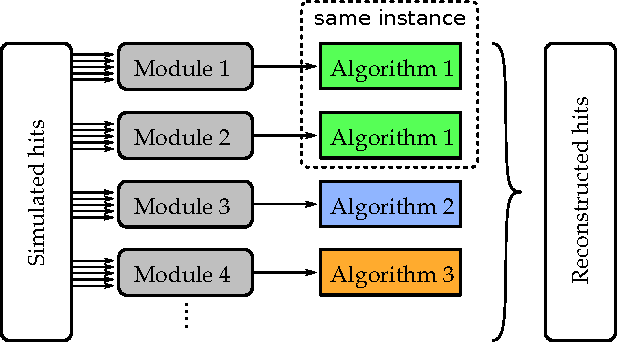
\includegraphics[scale=0.75]{figures/fastsim/parcels.pdf}
}

\subsection{Iterative tracking}

\myfigure{\label{fig:fsim-tracking}The track reconstruction workflow in \FSIM. Details are given in the text.}{
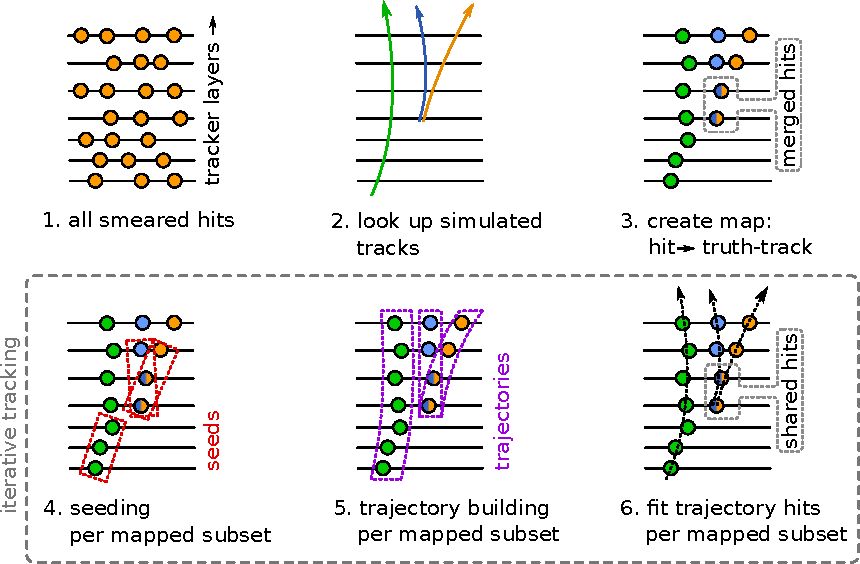
\includegraphics[scale=0.75]{figures/fastsim/tracking.pdf}
}

masking

\subsection{Seeding}

\myfigure{}{
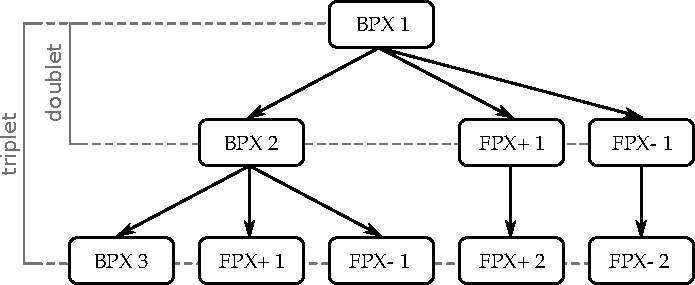
\includegraphics[scale=0.75]{figures/fastsim/seedingtree.pdf}
}

\subsection{Track fit}

\section{Validation}

\section{Conclusion}

%############################################################
\vspace{\baselineskip}
\hrule
\newpage
%############################################################

\section{Introduction}
Tracking of charged particles is one of the crucial ingredients to understand the physics behind LHC collisions. In the CMS experiment~\cite{Chatrchyan:2008aa}, tracks of charged particles are reconstructed and matched to information gathered by other subdetectors which improves the overall event reconstruction and resolution~\cite{CMS:2009nxa}. From reconstructed tracks higher analysis level objects like jets and the missing transverse energy are derived. 

Sophisticated tracking algorithms are required to reconstruct tracks from the large amount of charged particles transversing the CMS detector at each bunch crossing. At typical instantaneous luminosities of about $10^{34}\,\mathrm{cm}^{-2}\mathrm{s}^{-1}$, which was reached in 2016, more than 500 reconstructed tracks can originate from 20--30 proton-proton interactions per crossing.

The complex, multistep algorithms which reconstruct tracks from energy depositions left by traversing charged particles in the CMS tracker are very computing-intense. The standard track reconstruction procedure for data is applied to simulated events as well after they have passed the emulation of the electronic response of the detector. However, at this point in the simulation chain, it can be beneficial to sidestep the standard reconstruction by utilizing truth-information about the simulated events instead. In the CMS simulation framework this idea together with others has led to a fast alternative for simulating physics events called ``FastSimualtion'' (\FSIM[format=hyperbf]{})~\cite{fsimRahmat,fsimAndrea}. Such a fast alternative is further motivated in the light of the planned increase of luminosity for which larger samples of simulated events with higher pileup conditions have to be produced.

The goal of the \FSIM package of CMS, which is tightly integrated into the CMS software~\cite{Bayatian:922757}, is to provide a fast alternative to the standard simulation and reconstruction workflow while delivering high-level analysis objects with sufficient accuracy. This is achieved by sidestepping certain parts in the production of simulated event samples to achieve a significant speed up. The two major CPU-intense parts which are replaced are the Geant4-based~\cite{Agostinelli2003250} simulation of particle interactions with the detector material and the track reconstruction. The final analysis objects are indistinguishable from the ones produced by the standard simulation work flow. This enables an easy integration of \FSIM samples in analyses along samples from the standard simulation and data.

Nowadays, the \FSIM package is successfully employed within CMS analyses. Typical use cases are searches for beyond the standard model physics such as SUSY. Such analyses require usually multiple signal samples which reflect various realizations of a new physics model. Other use cases are the evaluations of the impact of systematic uncertainties on a measurement like a variation of the renormalization and factorization scales or the top quark mass. A more general use case is to enhance the statistics of existing samples for training multivariate analysis methods.

This article is organized as follows: First, the steps involved in the standard track reconstruction are described briefly. Then, their alternative implementation within the \FSIM package is detailed with an emphasis on new developments in its tracking emulation. After the validation where the tracking performance of the standard simulation and reconstruction is compared to \FSIM this article is summarized and an outlook on planned developments is provided.







\section{Standard track reconstruction within CMS}


The standard track reconstruction is applied to real data and to simulated events from the standard Geant4-based simulation. It begins with the forming of hits on the pixel and strip modules of the tracker. Dedicated templates of charge depositions from simulation are compared to data to infer the position of a hit on a pixel module~\cite{Swartz:2007zz}. On the strip modules, hits are seeded from strips and subsequently combined with adjacent ones if their readout is sufficiently above their noise level.

The reconstructed hits are then passed to the track reconstruction sequence which finds tracks iteratively. After each iteration the hits within the tracks that pass certain quality requirements are masked in next iterations to reduce the combinatorics. Currently, there are eight iterations deployed which will however be adapted after the upgrade of the pixel detector in 2017~\cite{Dominguez:1481838}. The first iterations target easy-identifiable, non-displaced tracks with respect to the interaction region, whereas the later iterations are designed for more complicated situations. Seeds are built from hit doublets or triplets on specific tracker layers which pass an iteration-dependent acceptance selection. Then, trajectories are constructed through the combinatorial track finder~(CTF) algorithm which tries to locate seed-compatible hits on other layers. It is based on Kalman filters and pattern recognition techniques.  Finally, the track parameters are estimated from a fit to the hit positions using a Runge-Kutta-based propagator which accounts for material effects and the inhomogeneous magnetic field. Tracks for analyses have to pass certain quality criteria depending on the iteration to reject ``fake'' tracks from spurious hit combinations. The fake rate is found to be about 5--15\% depending on the momentum and particle type in the standard simulation and reconstruction.

More information on the standard track reconstruction can be found in Ref.~\cite{Chatrchyan:2014fea}.


\section{Fast emulation of track reconstruction}

\todo{draw some image where fastsim is speeding things up}

In \FSIM, the simulation of energy loss of particles as they traverse the detector is performed using parameterized probability functions for emulating energy loss through ionization, nuclear scattering, and bremsstrahlung. No detailed information of charge deposition on the pixel and strip modules is generated. To mimic the resolutions of the standard hit reconstruction the true hit positions are smeared. A new \FSIM module for position smearing was recently developed which allows to manage various algorithms for position smearing side-by-side. It can be flexibly configured for any topology of the tracker. Additionally, each algorithm can be restricted to certain tracker modules only. Currently, a simple Gaussian smearing of the position is deployed for all strip modules where the configured resolution depends on the specific tracker subdetector and its layer. A more detailed emulation of hit reconstruction is employed for the pixel modules where parametrized distributions from the standard template-based hit reconstruction are utilized for the smearing. Furthermore, the new module allows the emulation of merging of two hits which occurs when the distributions of the deposited charge from two transversing particle overlap. Figure~\ref{fig:fsim-merge} shows a recent study of the probability of hit merging on the pixel modules. Such probability maps are expected to be used for the emulation of hit merging in the future.

\myfigure{\label{fig:fsim-merge}Probability of two hits merging on the pixel barrel modules as a function of their distance and local incident angle of a track expressed in pseudorapidity.}{
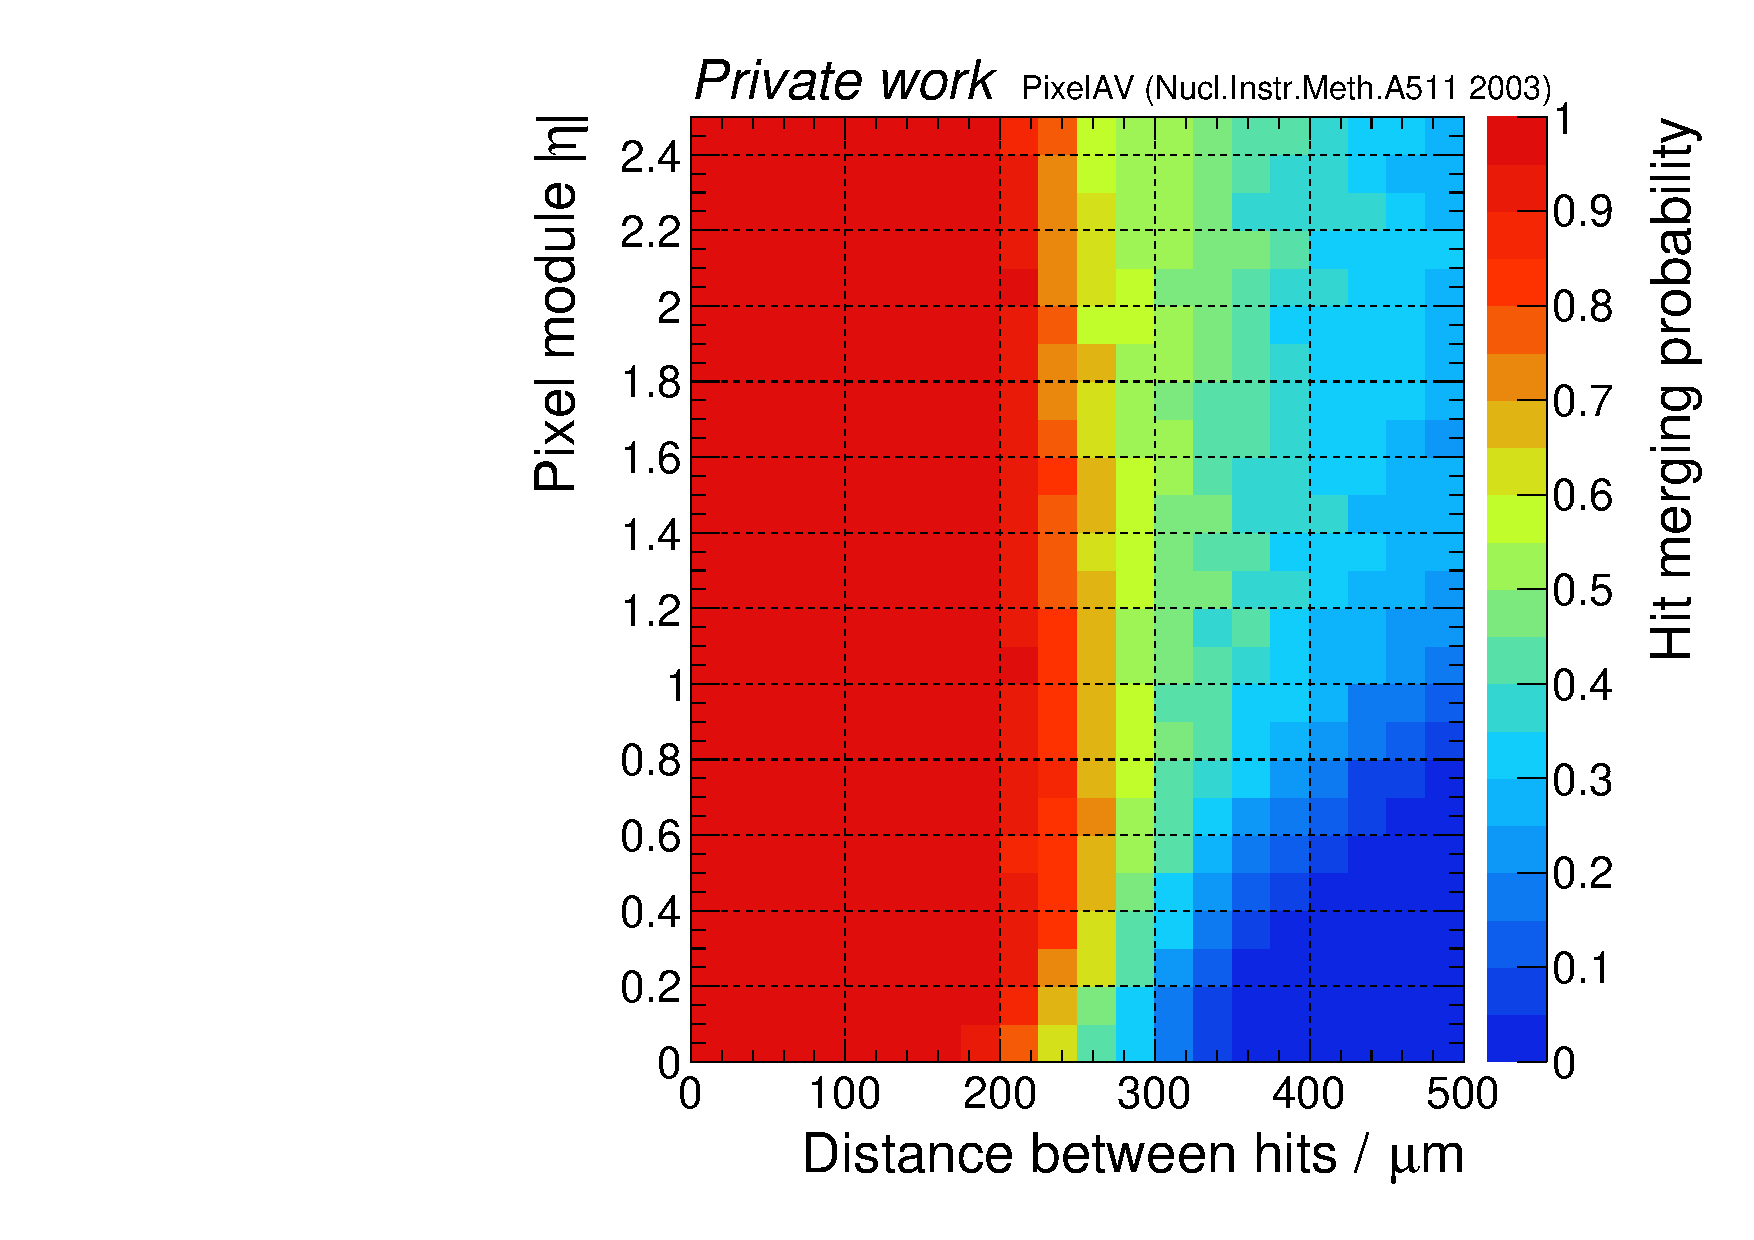
\includegraphics[width=0.48\textwidth]{figures/fastsim/merge.pdf}
}

By default, the seeding and trajectory building modules of the standard iterative tracking sequence are replaced completely within \FSIM. An overview is provided in Fig.~\ref{fig:fsim-tracking}. The ability to produce merged hits originating from close particle tracks necessitated a recent refactoring of the \FSIM{}-specific data objects within the iterative tracking sequence. As motivated in the introduction, the main idea of sidestepping the reconstruction by using truth information about the origin of each hit remains, but had to be extended. Instead of a one-to-one mapping of reconstructed hits to true particle tracks, close simulated hits can now result into a single reconstructed ``merged'' hit that can be shared between the final tracks within an iteration. A further benefit is that the mapping itself can be generated independently from the truth information which will allow the mix-in of wrong hit combinations leading to ``fake'' tracks in the future which are currently not emulated.

\myfigure{\label{fig:fsim-tracking}The track reconstruction workflow in \FSIM. Details are given in the text.}{
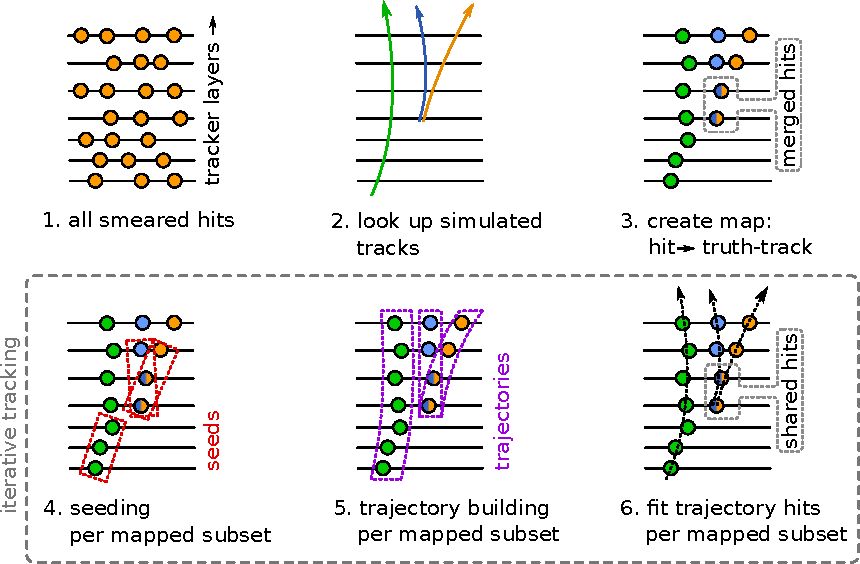
\includegraphics[width=0.99\textwidth]{figures/fastsim/tracking.pdf}
}

The seeding and trajectory building are restricted to the hits within a mapped subset. This removes completely any combinatorial problem from the iterative tracking in \FSIM resulting in a large reduction of computing time compared to the standard reconstruction. In the seeding step, the acceptance requirements are enforced by interfacing directly with the implemented criteria in the standard seeding step per iteration. The trajectory building process is trivial since the complete set of hits per track has already been defined. Finally, the track is fitted using the standard fit algorithm and the used hits are masked in next iterations.

For the simulation of pileup interactions, additional minimum bias events are first premixed according to the desired pileup scenario and then added to the events at random. In \FSIM, tracks are already reconstructed in premixed events and then included in the event directly without interfering with the hit and track reconstruction of the main interaction. In analyses, the reconstruction of primary vertices allows to differentiate between tracks stemming from the hard or pileup interactions via their vertex association which motivates this approach.


\section{Validation}

Track reconstruction within \FSIM is validated by comparing the tracks from the fast emulation with those obtained from the Geant4-based simulation and standard reconstruction. Figure~\ref{fig:fsim-eff-tracks} presents the tracking efficiency as a function of the transverse momentum and pseudorapidity. Here, the tracking efficiency is defined as the ratio of reconstructed tracks matched to simulated charged particles over the total number of charged particles within the tracker volume. Furthermore, the obtained resolution of the transverse momentum for reconstructed tracks is shown in Fig.~\ref{fig:fsim-res-track}. Overall, the plots demonstrate a good agreement of the \FSIM tracking performance with the one observed in the Geant4-based simulation and standard reconstruction.

\myfigure{\label{fig:fsim-eff-tracks}Comparison of the reconstruction efficiencies of tracks as a function of (a)~the transverse momentum and (b)~the pseudorapidity measured in the simulation of top quark pair production at 13~TeV.}{
\subfloat[]{\centering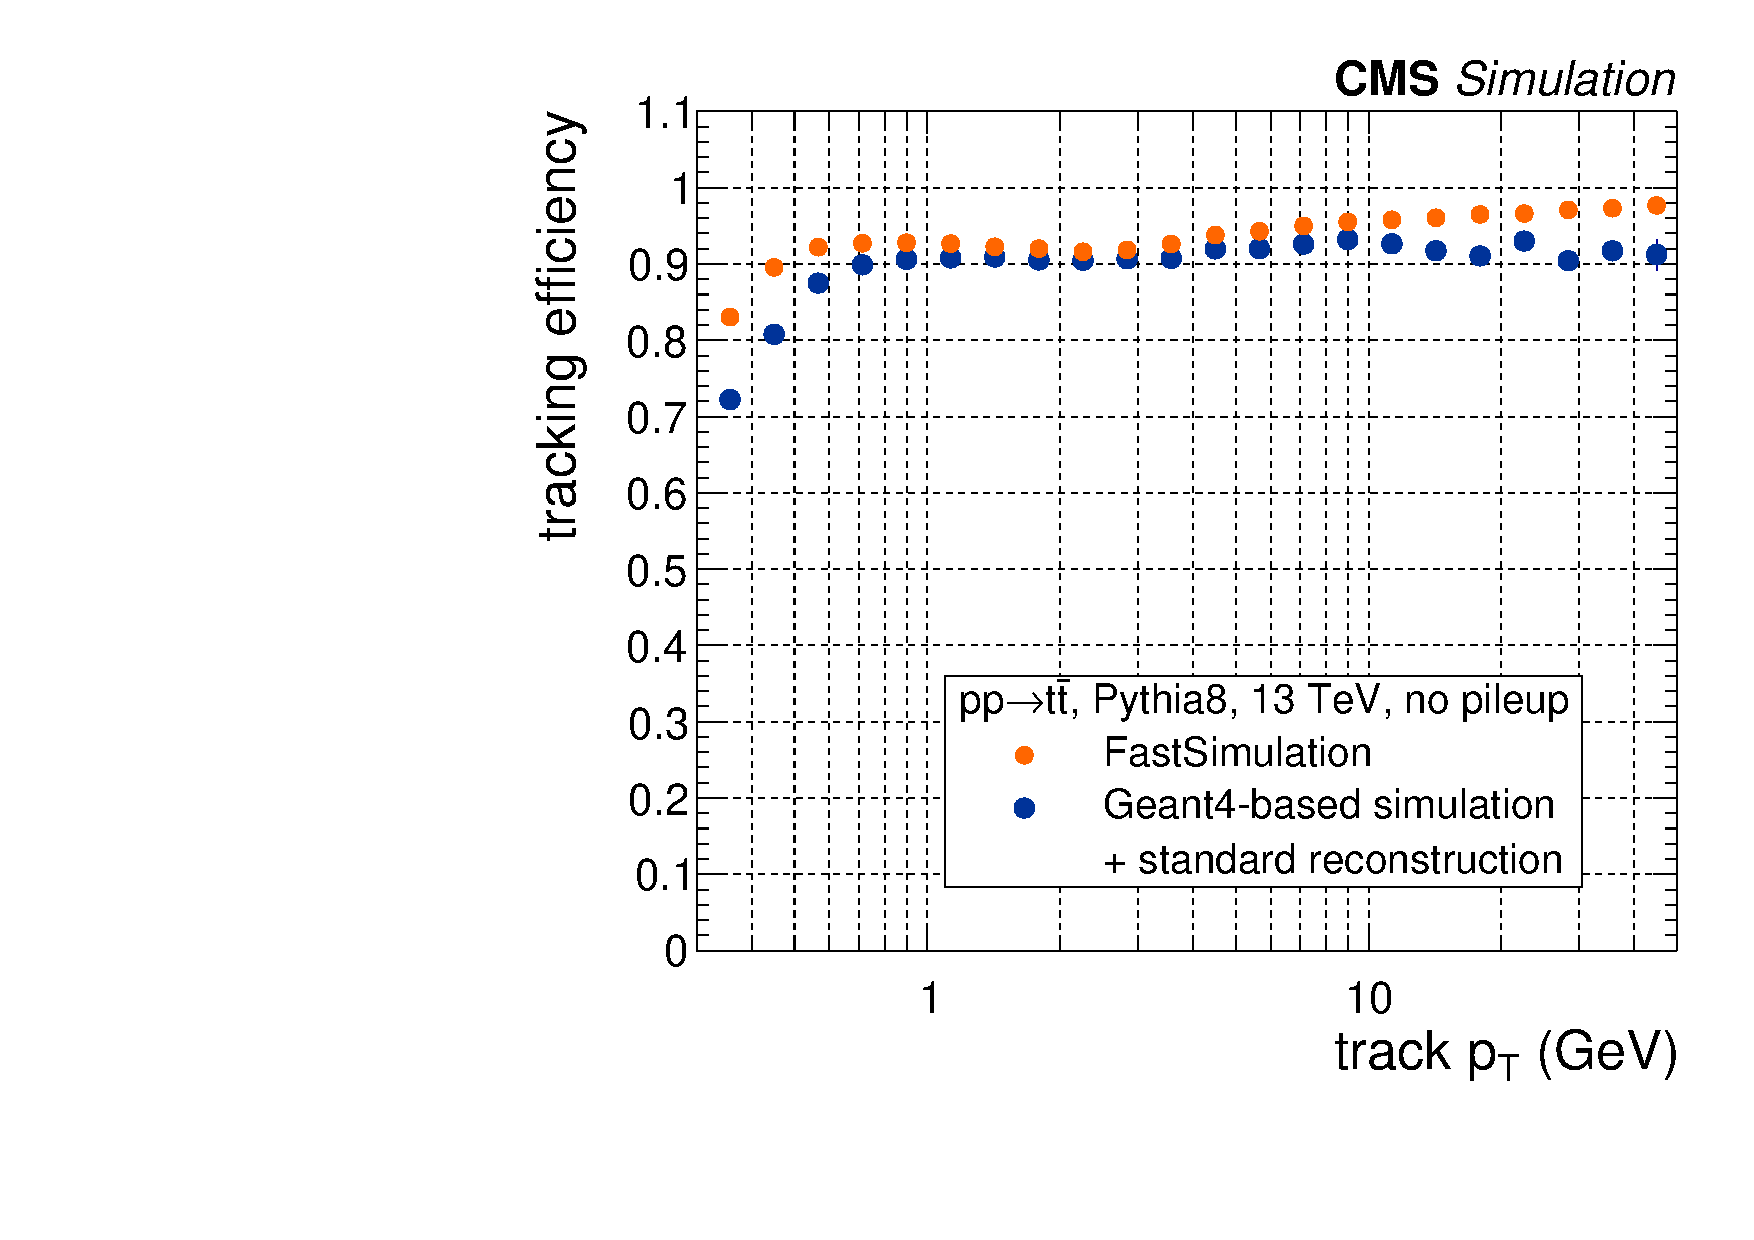
\includegraphics[width=0.48\textwidth]{figures/fastsim/eff_pt.pdf}}
\hspace{0.02\textwidth}
\subfloat[]{\centering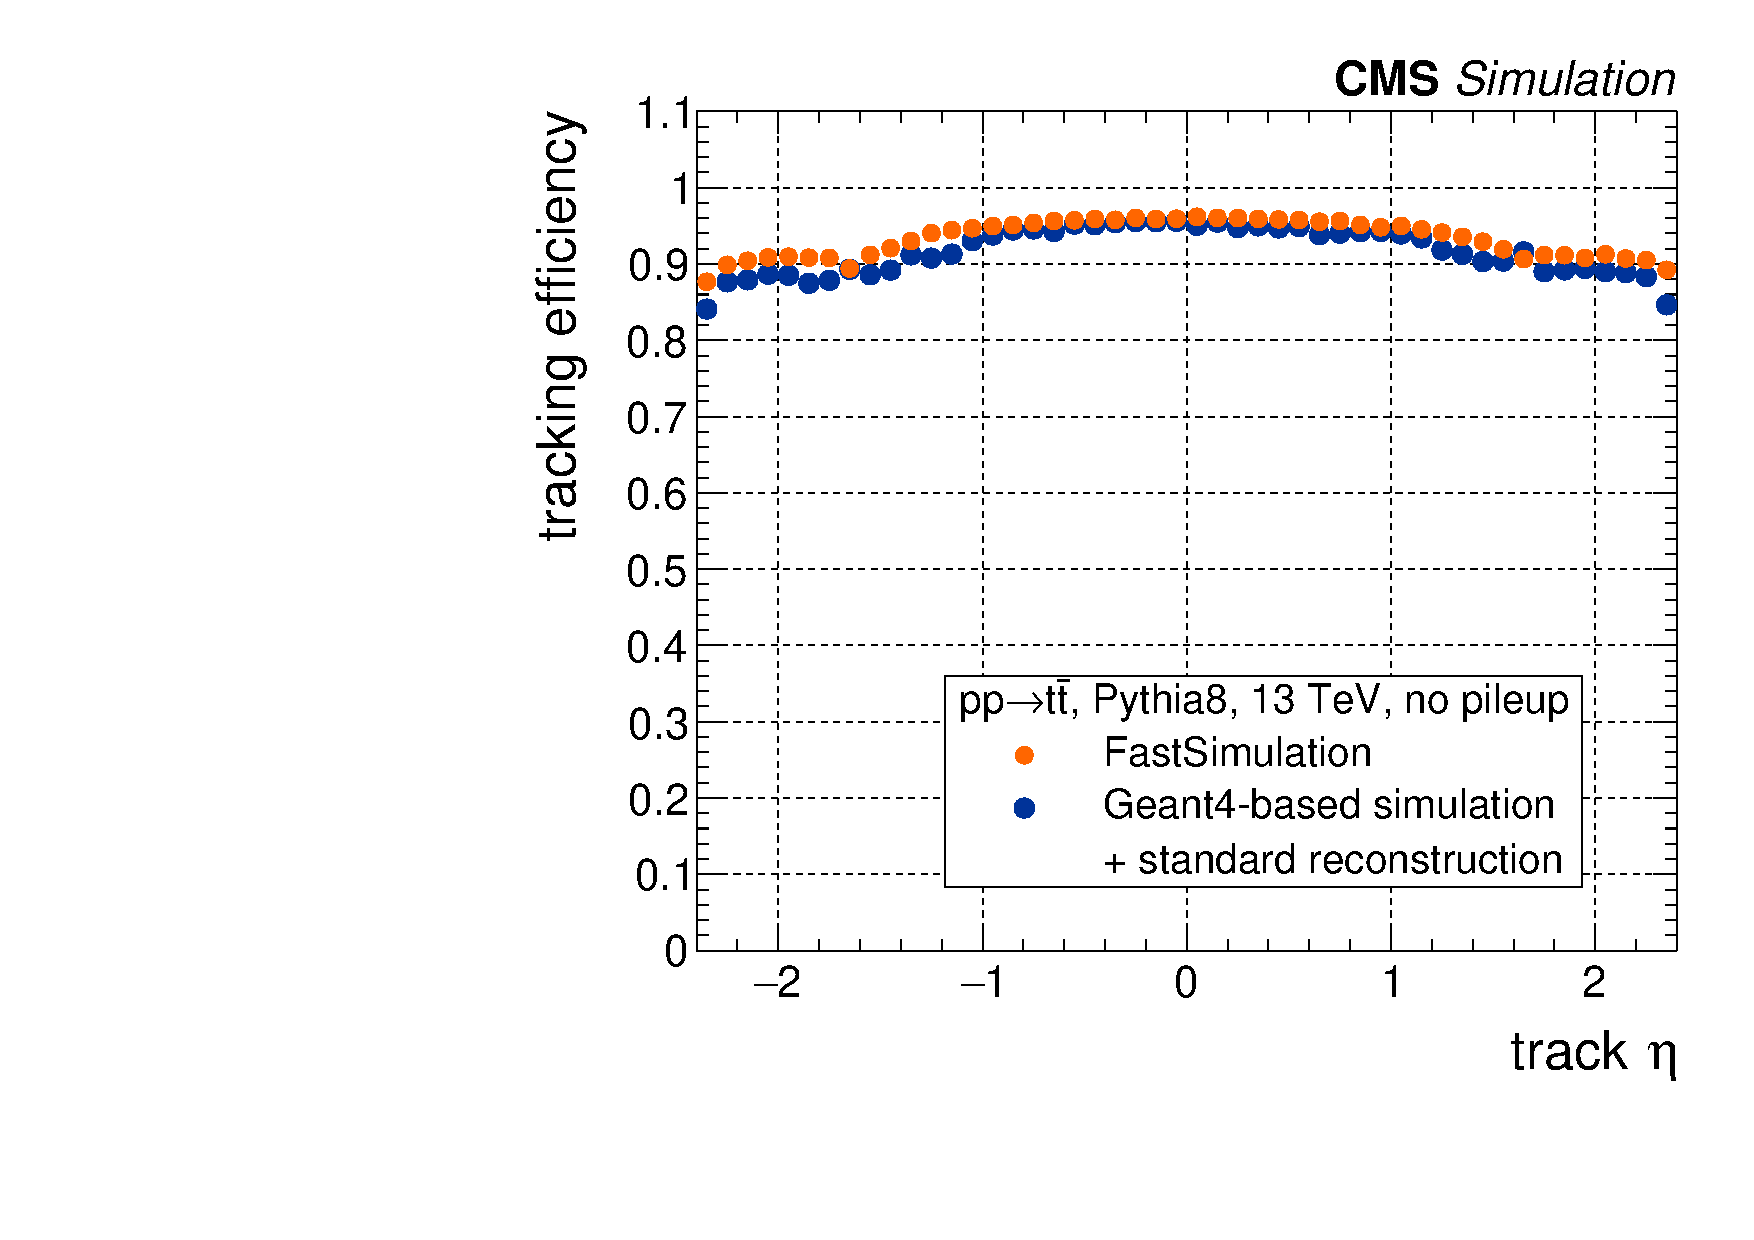
\includegraphics[width=0.48\textwidth]{figures/fastsim/eff_eta.pdf}}
}

A profile of the average CPU-time consumption per event within \FSIM is given in Fig.~\ref{fig:fsim-cpu} as a function of the average number of pileup interactions. Less than 10~s are required to simulated an event of top quark pair production for current pileup scenarios with $\approx30$ interactions on average. The emulation of tracking is not amongst the top CPU consumers.

\myfigure{\label{fig:fsim-res-track}Comparison of the resolution of reconstructed tracks as a function of the transverse momentum measured in the simulation of top quark pair production at 13~TeV.}{
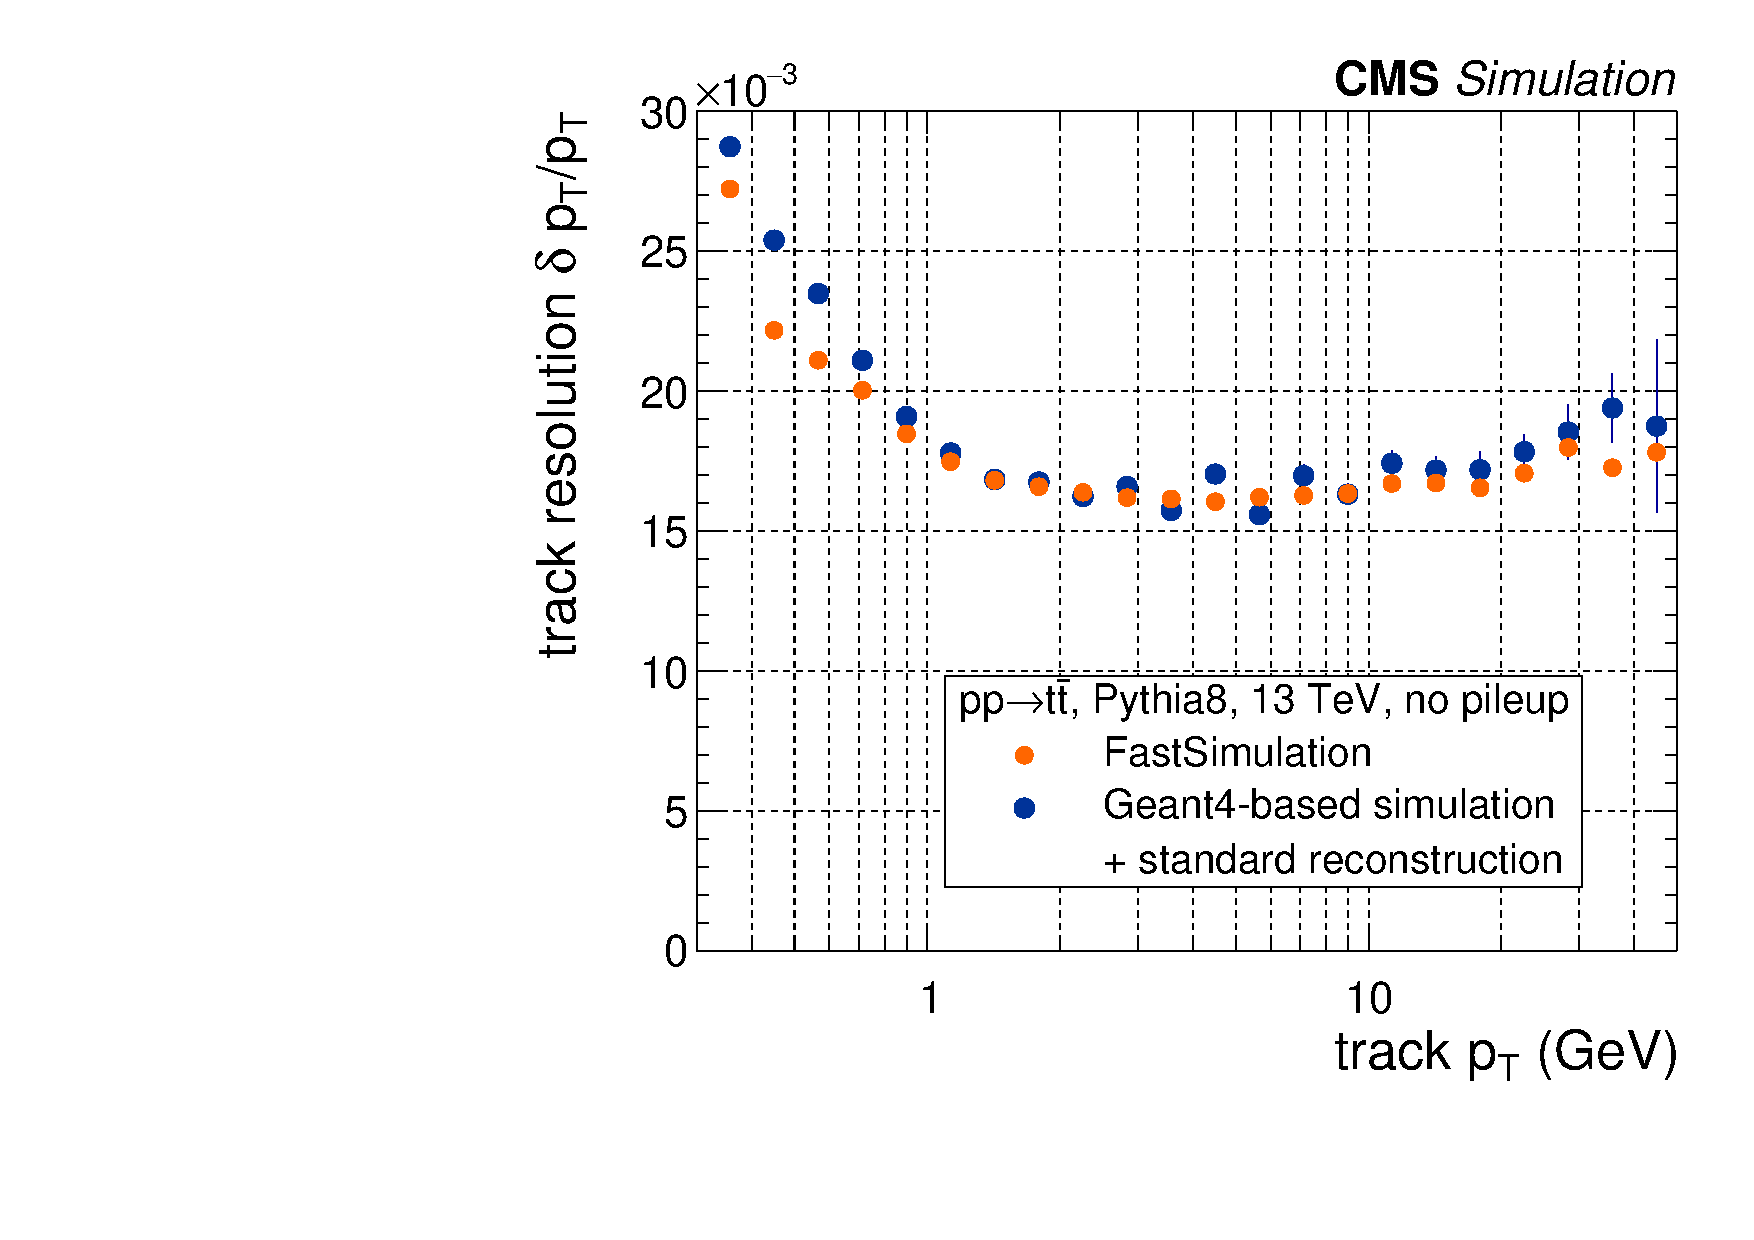
\includegraphics[width=0.48\textwidth]{figures/fastsim/res_pt.pdf}
}

\myfigure{\label{fig:fsim-cpu}Average CPU-time per event spent on the detector simulation and the reconstruction of analysis objects as a function of the average number of pileup interactions measured in the simulation of top quark pair production at 13~TeV.}{
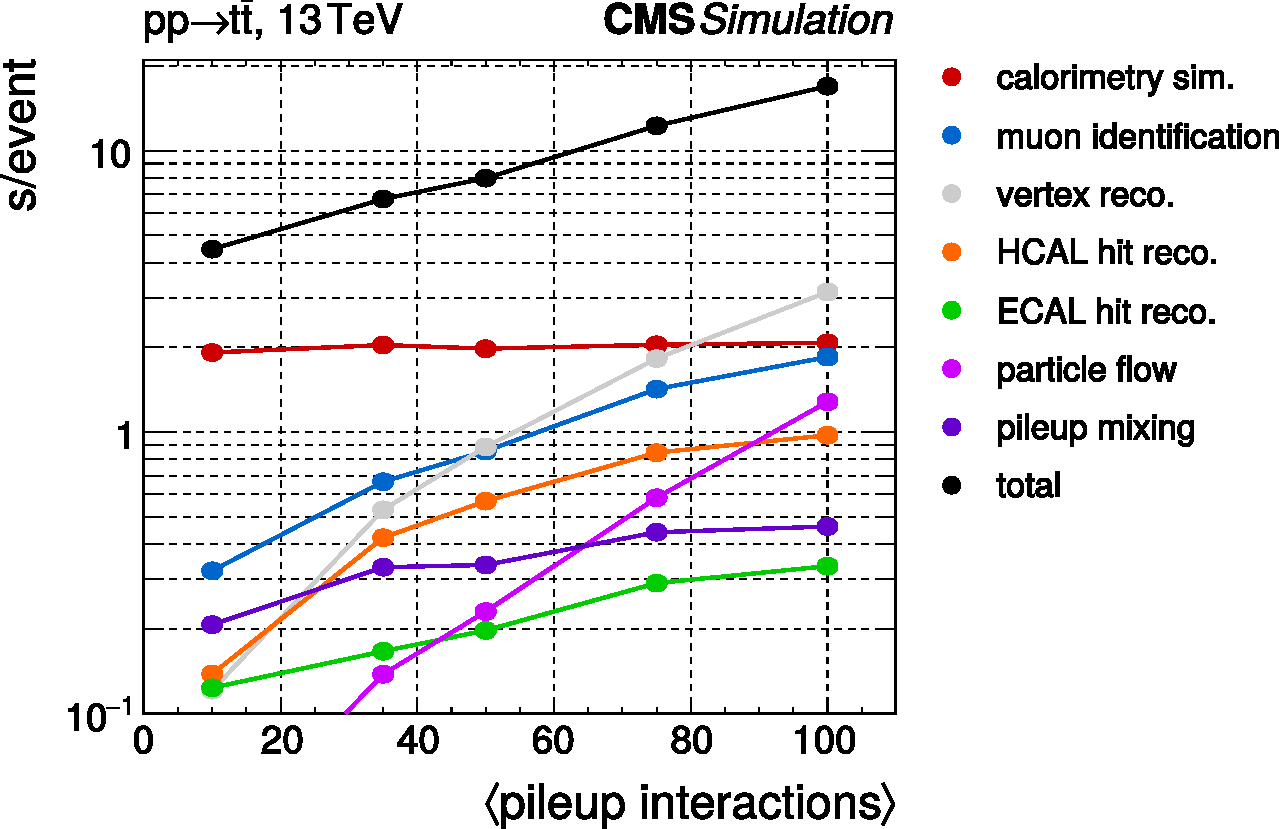
\includegraphics[width=0.6\textwidth]{figures/fastsim/cpu_profile.pdf}
}

\section{Conclusion and outlook}

The CMS \FSIM package provides a fast alternative to the standard simulation and reconstruction workflow. One of its major speedups is the use of truth information in the track reconstruction. Recent developments in the framework led to further flexibility in the emulation of hit reconstruction and to the usage of truth information in the iterative tracking sequence. In the short term, these developments will enable the emulation of the emulation of merged hits originating from close particle tracks. In the long term, the increased flexibility will allow to adapt the emulation of track reconstruction to the planned upgrades of the CMS detector.

